\section{Reachi Experiments}\label{sec:reachi-experiments}
\todo[inline]{describe angel approach, ref old report}

Packet loss is a real world phenomenon that our simulations need to include to increase quality of the simulations. In \cite{paper:sims1} an approach for computing path loss is described, were the computation is done in two parts:

\begin{description}
    \item[$\vect{l_d}$] A determistic distance dependent part, that computes path loss based on the distance of the link~\cite[p.~6]{paper:sims1}. $l_d$ can be seen on \autoref{eq:ld}~\cite[p.~29]{paper:linkmodel}.
    \item[$\vect{l_{\mathit{fading}}}$] A stochastic slow/shadow fading part, which specifies the local mean of the signal, in dB.
    The slow fading variable is, more or less, constant in the same local area, as it is caused by terrain, buildings, vegetation, and cars. It is a vector of size n, where n is the number of links in the network~\cite[p.~6]{paper:sims1}.
\end{description}


\begin{eq}\label{eq:ld}
    l_d(l) = 10 \gamma log_{10}(d(l)) - c
\end{eq}
$d(l)$ is a function returning the distance of a link, the path loss exponent $\gamma = 5.5$, the costant offset $c = -18.8$. The constants used in $l_d$ were computed with \gls{tls}~\cite[p.~25]{paper:linkmodel}.\medbreak

$l_{fading}$ introduces stochastic path loss, to simulate the random loss off signal strength caused by the environment from buildings, trees etc. In~\cite{paper:linkmodel} this was done with an angle based approach. The assumption is that if two links has a small angle between them, i.e. a high correlation, the path loss introduced from the environment is close to the same. In~\cite{paper:sims1} this approach was implemented and tested, but faulty and gave bad results. Further details why can be read in~\cite{paper:sims1}.


\todo[inline]{introduce the data. WIP}
As part of this project, we received logs from field experiments from the Reachi project. Field experiments were conducted in diffrent locations with their prototypes, collecting information about their \gls{gps} coordinates at a given time, and the current neighbourhood at the time in 20 seconds intervals. The \gls{rssi} to each neighbour was collected with the neighbourhood information. The logs are to be used as comparison to our simulations, to verify that the simulations give a similar log.


\todo[inline]{talk about the problems with the data and angle approach. WIP}
Close examination of the logs has shown problems with the angle based approach and the distance dependent part $l_d$. \autoref{plot:reachi-experiments:measurements-vs-ld} plots samples drawn from $l_d$ and measurments from the Marikina log. Since the log contained a total of 17761 links throughout the whole field test, the measurements are summarised based on the distance of the links. Each link was sorted into distance buckets with 20 meters interval i.e. links with a distance between 20 meters and 40 meters were sorted together, up to 740 meters as that was the longest link in the log. The average \gls{rssi} for all links in each bucket was then computed. \autoref{plot:reachi-experiments:measurements-vs-ld} shows that the $l_d$ does not fit with the measurements and as such not usable for our simulations.

\begin{figure}[H]
    \centering
    \begin{tikzpicture}
        \begin{axis}[
                height=12cm, width=0.95\textwidth,
                ylabel={RSSI},
                xlabel={Distance in meters},
                axis lines*=left,
                xmin=0, xmax=750,
                enlargelimits=false,
                ymin=-120, ymax=-20,
                xtick={0, 50, 100, 150, 200, 250, 300, 350, 400, 450, 500, 550, 600, 650, 700, 750},
                ymajorgrids=true,
                xmajorgrids=true,
                grid style=dashed,
                restrict y to domain=-120:-20,
                samples=600
            ]

            \addplot[very thick, solid, cyan, mark=*] coordinates {(20, -28.32345013477089) (40, -44.85830258302583) (60, -52.77323717948718) (80, -60.21201657458563) (100, -66.47435897435898) (120, -69.68905472636816) (140, -71.5976496922216) (160, -73.7866473149492) (180, -75.53428571428572) (200, -76.89289392378991) (220, -77.88135593220339) (240, -77.8035019455253) (260, -77.36784140969164) (280, -77.14030612244898) (300, -77.75299760191847) (320, -79.71686746987952) (340, -79.15481171548117) (360, -79.90728476821192) (380, -81.30909090909091) (400, -81.79746835443038) (420, -81.52272727272727) (440, -79.2) (460, -79.42105263157895) (480, -79.4375) (500, -79.0) (520, -77.91666666666667) (540, -83.0) (560, -81.27272727272727) (580, -83.57142857142857) (600, -86.0) (620, -83.4) (640, -86.5) (660, -81.42857142857143) (680, -79.0) (700, -82.71428571428571) (740, -77.0)};
            \addlegendentry{Marikina field measurements};


            \addplot[domain=0:740, very thick, solid, red] {26 - ld(x)};
            \addlegendentry{$l_d$\cite[p.~29]{paper:linkmodel}};
        \end{axis}
    \end{tikzpicture}
    \caption{Average RSSI pr. distance}\label{plot:reachi-experiments:measurements-vs-ld}
\end{figure}


As mentioned above, the angle based approach relies on the assumption that link pairs with a high correlation, i.e. low angle between them, will have close to the same shadow fading. We have however not been able to produce reliable proof that the assumption is correct. To produce proof, the Marikina and Rude skov log was used. For both logs, link pairs were created and sorted based on their angle into separate bucekts of 5$\degree$ intervals. The average \gls{rssi} for each bucket was then computed. Before computing the average \gls{rssi}, the distance dependent part $l_d$ was removed from the links \gls{rssi} measurement, to isolate the stochastic part. The resulting data can be seen plotted on \autoref{plot:reachi-experiments:avg-rssi-angle-phili-rude}. Under the previous assumption that a high correlation gives smaller stochastic path loss, then the traces on \autoref{plot:reachi-experiments:avg-rssi-angle-phili-rude} should increase gradually as the angle increases. Clearly the measurements does increase as the angle increase, but the increaes are not steady but rather vary greatly. Too greatly to say that with certainty that the assumption holds on the received logs.

\todo[inline]{fix plot}
\begin{figure}[H]
    \centering
    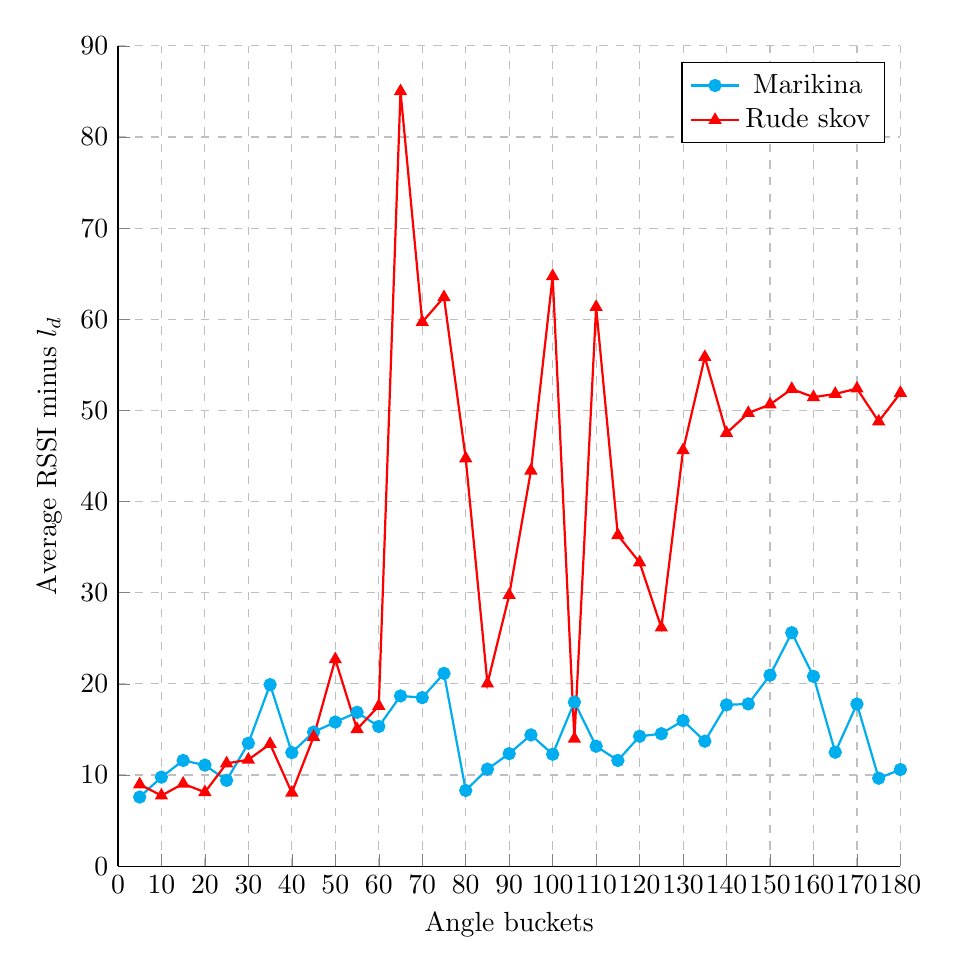
\begin{tikzpicture}
        \begin{axis}[
                height=12cm, width=0.95\textwidth,
                ylabel={Average RSSI minus $l_d$},
                xlabel={Angle buckets},
                axis lines*=left,
                xmin=0, xmax=180,
                xtick={0, 10, 20, 30, 40, 50, 60, 70, 80, 90, 100, 110, 120, 130, 140, 150, 160,170,180},
                enlargelimits=false,
                ymin=0, ymax=90,
                ymajorgrids=true,
                xmajorgrids=true,
                grid style=dashed
            ]

            \addplot[thick, solid, cyan, mark=*] coordinates {(5,7.581215097994852)(10,9.763581254686114)(15,11.59234807189617)(20,11.084399582147876)(25,9.411670936293284)(30,13.486232393853125)(35,19.91110051641767)(40,12.453590557884946)(45,14.70313120243339)(50,15.804939314638208)(55,16.87697870999425)(60,15.320902904198922)(65,18.673392004683087)(70,18.48508963612783)(75,21.147550183881993)(80,8.302184073487094)(85,10.641508684206432)(90,12.343183048128944)(95,14.396643466792797)(100,12.27504884861337)(105,17.994872329043496)(110,13.156645245862158)(115,11.595967499573286)(120,14.245146945189493)(125,14.528392002600814)(130,15.96981736460891)(135,13.70427190114752)(140,17.692009757218077)(145,17.79486440192431)(150,20.947579654378668)(155,25.611175147469265)(160,20.819124899373364)(165,12.495568407794714)(170,17.784042978338544)(175,9.646875797269503)(180,10.597197732034614)};
            \addlegendentry{Marikina};


            \addplot[thick, solid, red, mark=triangle*] coordinates {(5,8.968175725354994)(10,7.741408675352775)(15,9.042742837449076)(20,8.108954051047618)(25,11.273321343260399)(30,11.67692967914715)(35,13.401460743255232)(40,8.053793318539391)(45,14.17474549040368)(50,22.68855220716477)(55,15.026896145186285)(60,17.5755161176863)(65,85.01233086400362)(70,59.69038212814202)(75,62.41948703096457)(80,44.72712810089782)(85,20.029080610052482)(90,29.737954905927445)(95,43.39235466255519)(100,64.720015835849)(105,13.965589072181558)(110,61.334883149884675)(115,36.30455538419785)(120,33.32223486902817)(125,26.172354285886417)(130,45.62355888699502)(135,55.8474401182669)(140,47.511612928722954)(145,49.70429537245245)(150,50.649080550831435)(155,52.34402139529124)(160,51.45218633523966)(165,51.805898996936115)(170,52.39131328924595)(175,48.78102582759046)(180,51.91529108595685)};
            \addlegendentry{Rude skov};
        \end{axis}
    \end{tikzpicture}
    \caption{}
    \label{plot:reachi-experiments:avg-rssi-angle-phili-rude}
\end{figure}